\subsection{Campo guia}
Pelo principio da inércia de Newton, um corpo tende a permanecer em movimento retilínio uniforme se não há forças que o obriguem a mudar sua trajetória. Logo, para que o elétron tenha uma órbita circular, é necessário aplicar uma força que mude sua trajetória da forma desejada.

Pela força de Lorentz,
\begin{align}
	\vec{F} = q\left(\vec{E} + \vec{v} \times \vec{B}\right)
\end{align}
onde $q$ é a carga da partícula em movimento, $\vec{E}$ é o vetor de campo elétrico, $\vec{v}$ é o vetor de velocidade da partícula e $\vec{B}$ é o vetor de campo magnético.

A contribuição referente à força elétrica ($q\vec{E}$) é paralela ao campo elétrico, enquanto a contribuição referente à força magnética ($q(\vec{v}\times\vec{B})$) é perpendicular ao campo magnético e à velocidade. Devido a este fato, a força magnética não realiza trabalho, uma vez que é perpendicular ao deslocamento da partícula. Logo, a força magnética altera a direção do vetor velocidade -- e, por consequência, do movimento da partícula -- sem alterar o seu módulo. Apenas a força elétrica pode realizar trabalho.

Desta forma, a fim de desviar a partícula da sua trajetória, aplica-se um campo magnético $\vec{B}$ nos pontos onde ela deve fazer alguma curva, o qual é chamado de campo guia. Com $E=0$,
\begin{align}
	\vec{F} = q\vec{v}\times\vec{B}
\end{align}

Espera-se que a órbita ideal ocorra no plano horizontal ($z=0$) de forma que o campo magnético deve ser puramente vertical em toda a órbita do anel. Considerando o campo magnético simétrico com relação ao plano da órbita ideal e fazendo uma aproximação linear, pode-se escrever a equação do campo magnético através da expansão de Taylor:
\begin{align}
	B_z(s,x,z) &= B_0(s) + \left(\frac{\partial B_z}{\partial x}\right)_{0s} x\label{eq:2.01}\\
	B_x(s,x,z) &= \left(\frac{\partial B_x}{\partial z}\right)_{0s} z\label{eq:2.02}
\end{align}

Pela simetria imposta, aplicando as leis de Maxwell,
\begin{align}
	\frac{\partial B_z}{\partial x} = \frac{\partial B_x}{\partial z}
\end{align}

Desta forma, as equações \eqref{eq:2.01} e \eqref{eq:2.02} podem ser reescritas como
\begin{align}
	B_z(s,x,z) &= B_0(s) + \left(\frac{\partial B}{\partial x}\right)_{0s} x\label{eq:2.1}\\
	B_x(s,x,z) &= \left(\frac{\partial B}{\partial x}\right)_{0s} z\label{eq:2.0}
\end{align}

Como o campo é simétrico em relação ao plano da órbita ideal, as variáveis $B_0$ e $\frac{\partial B}{\partial x}$ possuem apenas componentes verticais, então apenas suas magnitudes são necessárias para descrevê-las completamente e os índices $s$ e $z$ podem ser suprimidos.

Anéis de armazenamento são modelados para operar em uma faixa de valores de energia dos elétrons. Isto é obtido arranjando de forma que os campos magnéticos possam ser variados juntos -- sendo parametrizados proporcionalmente à energia de operação desejada. Claramente, se o campo magnético na órbita ideal é mudado em todo o anel pelo mesmo fator, a órbita ideal será, novamente, uma trajetória possível de um elétron cujo momento é mudado pelo mesmo fator. Variar todos os campos juntos altera muito pouco a energia associada com a órbita ideal. Por essas razões, é conveniente especificar as propriedades do campo guia de uma maneira que seja independente de qualquer energia de operação escolhida, o que é facilmente feito dividindo todos os campos por um fator proporcional à energia associada do elétron, o qual é chamado de rigidez magnética. Desta forma, as propriedades lineares do campo guia podem ser definidas pelas funções
\begin{align}
	G(s) &= \frac{ecB_0(s)}{E_0}\\
	K_1(s) &= \frac{ec}{E_0} \left(\frac{\partial B}{\partial x}\right)_{0s}
\end{align}
onde $E_0$ é a energia nominal, $c$ é a velocidade da luz e $e$ é a carga do elétron. Note que estas funções tem um significado físico bem simples. Neste caso, apenas elétrons ultra-relativísticos são considerados, então sua energia é dada por $E=cp$. Desta forma, $G(s)$ é apenas o inverso do raio de curvatura $\varrho(s)$ dos elétrons em $x=0$ e $z=0$ com energia nominal, ou seja,
\begin{align}
	G(s) = \frac{1}{\varrho(s)}
\end{align}

\begin{proof}
	Como a partícula está rotacionando sobre ação da força de Lorentz, esta força deve ser equivalente a sua força centrípeta. Logo,
	\begin{align*}
		\frac{mv^2}{\varrho(s)} &= q\vec{v}\times\vec{B}\\
							    &= evB_0(s)\\
	\end{align*}
	
	Como o elétron é ultra-relativístico (com velocidade próxima/igual à velocidade da luz), a energia da partícula é dada por
	\begin{align*}
		E_0^2 = (m_0 c^2)^2 + p^2c^2
	\end{align*}
	onde $m_0$ é a massa de repouso e $p$ o momento da partícula. Pelo mesmo argumento anterior, $(m_0c^2)^2 << c^2p^2$. Desta forma, pode desprezar o termo $(m_0c^2)^2$ e a energia da partícula é dada por
	
	\begin{align*}
		E_0 &= pc\\
			&= \gamma m_0 c^2\\
			&= mc^2
	\end{align*}
	
	Substituindo,
	\begin{align*}
			\frac{mv^2}{\varrho(s)} &= ecB_0(s)\\
			\frac{E_0}{\varrho(s)} &= ecB_0(s)\\
			\therefore \frac{1}{\varrho(s)} &= \frac{ecB_0(s)}{E_0} = G(s)
	\end{align*}
	
	Desta forma, reescrevendo a equação do campo magnético em função de $G(s)$,
	\begin{align*}
		B_z(s,x,z) &= B_0(s) + \frac{\partial B}{\partial x} x\\
				   &= \frac{E_0}{ec} G(s) + \frac{\partial B}{\partial x} x
	\end{align*}
	
	Definindo a função $K_1(s)$ como
	\begin{align*}
		K_1(s) = \frac{ec}{E_0} \frac{\partial B}{\partial x}
	\end{align*}
	tem-se que
	\begin{align*}
		B_z(s,x,z) &= \frac{E_0}{ec} G(s) + \frac{\partial B}{\partial x} x\\
				   &= \frac{E_0}{ec} G(s) + \frac{E_0}{ec} K_1(s) x\\
				   &= \frac{E_0}{ec} [G(s) + K_1(s) x]
	\end{align*}
	Reescrevendo $B_x(s,x,z)$ da mesma forma, as equações do campo magnético são
	\begin{align*}
		B_z(s,x,z) &= \frac{E_0}{ec} [G(s) + K_1(s) x]\\
		B_x(s,x,z) &= \frac{E_0}{ec} K_1(s) z
	\end{align*}
\end{proof}

A constante de proporcionalidade $\frac{E_0}{ec}$ é a rigidez magnética do anel de armazenamento. Ela normaliza as equações do campo magnético de forma que este dependa apenas das propriedades da ótica do anel.

Devido à relação entre $G(s)$ e $\varrho(s)$, $G(s)$ é chamada de função de curvatura. A função $K_1(s)$ é a taxa de variação do raio inverso com o deslocamento radial.

As funções $G(s)$ e $K_1(s)$ podem ser arbitrárias, porém devem satisfazer alguns requisitos importantes. Primeiro, $G(s)$ precisa ser tal que esta defina uma órbita fechada (pode-se pensar que $G(s)$ define a órbita ideal, ou que alguma órbita fechada arbitrária define $G(s)$ de forma única). A variação $d \theta_0$ na direção da tangente à órbita ideal em um intervalo $ds$ é
\begin{align}
	-d\theta_0 = \frac{ds}{\varrho(s)} = G(s)ds
\end{align}

O ângulo percorrido em uma revolução precisa ser igual a $2\pi$, então $G(s)$ deve satisfazer
\begin{align}
	\int_{0}^{L} G(s)ds = 2\pi
\end{align}

Segundo, tanto $G(s)$ quanto $K_1(s)$ são, necessariamente, funções periódicas de $s$, devido ao fato de que a coordenada longitudinal $s$ é fisicamente cíclica -- retornando ao mesmo ponto da órbita após uma revolução. Dito isso, $G(s)$ e $K_1(s)$ também devem satisfazer
\begin{align}
	\left\{\begin{array}{rcl}
	\ G(s+L) & = & G(s)\\
	K_1(s+L) & = & K_1(s)
	\end{array}\right.
\end{align}
onde $L$ é o comprimento da órbita. Execeto por estas condições, $G(s)$ e $K_1(s)$ podem ter mais ou menos variações arbitrárias com $s$.

Apesar das funções do campo guia $G$ e $K_1$ serem, a princípio, bem gerais, geralmente é conveniente simplificar o design ou a operação de um anel de armazenamento impondo certas restrições nestes aspectos. Por exemplo, a maioria dos anéis de armazenamento são desenhados para ter o mesmo raio de curvatura, diga-se $\varrho_0$, em todos os ímãs de curvatura -- e sem nenhuma curvatura entre um ímã e outro, ou seja, apenas trechos retos. Este tipo de campo guia é chamado isomagnético. O intuito desta configuração é que o campo magnético sobre a órbita ideal tenha o mesmo valor em todo lugar, exceto onde este é nulo. Então $G(s)$ é uma função dicotômica:
\begin{align}
	G(s) = \left\{\begin{array}{rrrr}
	\ G_0 & = & \frac{1}{\varrho_0}, &  no\ \acute{i}m\tilde{a}\\
	0, & & & em\ todo\ o\ resto
	\end{array}\right.
\end{align}

Um campo guia real não pode, claro, ser idealmente isomagnético, já que é fisicamente impossível ter um campo magnético descontínuo. Sempre há uma zona de transição nas bordas do ímã onde o campo vai de zero ao seu valor nominal. A aproximação isomagnética ideal é, entretanto, um tanto quanto adequada no geral.

Apesar de aceleradores e anéis de armazenamento comumente serem construídos com ímãs de curvatura com gradientes radiais de campo, é comum desenvolver campos guia de função separável, ou seja, campos magnéticos em que as funções de focalização e curvatura são atribuídas a elementos magnéticos diferentes. Isto é, o campo guia consiste numa sequência de dipolos (sem gradiente de campo) e quadrupolos (sem campo na órbita ideal). Pensando nesta configuração, define-se um campo guia de função separável onde as funções $G(s)$ e $K_1(s)$ devem satisfazer a condição
\begin{align}
	G(s)K_1(s) = 0\label{eq:2.10}
\end{align}

Um pouco de atenção para este fato. Às vezes é conveniente projetar os ímãs de curvatura com faces retangulares. Com este tipo de ímã, a órbita ideal deve entrar ou sair do ímã com um ângulo diferente de 90$^\circ$ em relação à borda do mesmo (Figura \ref{fig:fig8}). Mesmo que o ímã seja plano (sem gradiente radial no ímã), irão existir gradientes radiais nas bordas, onde o campo não é nulo. A equação \eqref{eq:2.10} não é satisfeita nas bordas, e um campo guia construído com estes ímãs retangulares -- junto com os quadrupolos -- não irá satisfazer a definição de função separável, mesmo que ele seja referenciado como tal às vezes. Estes campos ainda podem ser, entretanto, isomagnéticos. 

\begin{figure}[!htb]
	\centering
	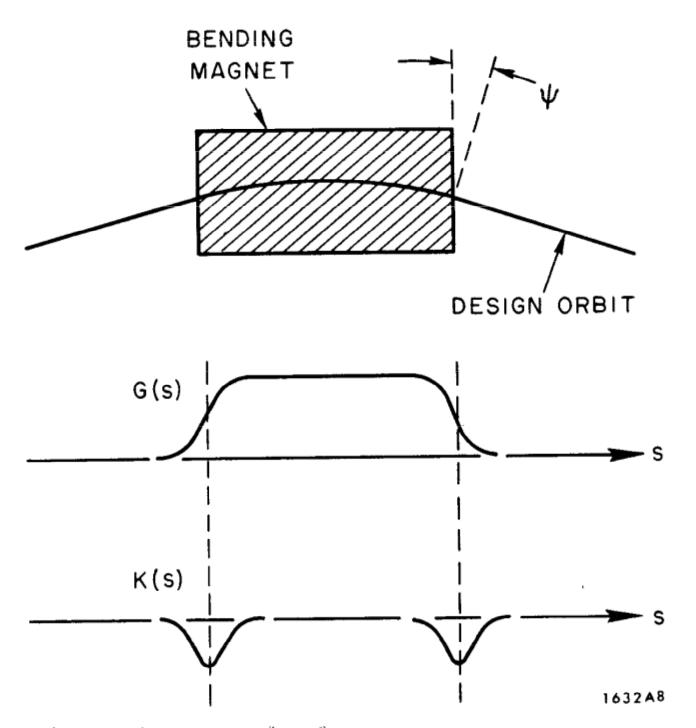
\includegraphics[width=0.6\linewidth]{./Figuras/fig8.jpeg}
	\caption{Campo guia com ímã retangular. Retirado de \cite{sands1970physics}.}
	\label{fig:fig8}
\end{figure}